
\documentclass[12pt,a4paper]{article}
\usepackage{geometry}
 \geometry{
 a4paper,
 total={170mm,257mm},
 left=20mm,
 top=20mm,
 }
\usepackage[utf8]{inputenc}
\usepackage[T1]{fontenc}
%\geometry{verbose,tmargin=3cm,bmargin=2cm,lmargin=2cm,rmargin=2cm,headheight=2cm,headsep=2cm,footskip=2cm}
\usepackage{array}
\usepackage{float}
\usepackage{textcomp}
\usepackage{slashed}
\usepackage{amsmath}
\usepackage{graphicx}
\usepackage{tikz}

\makeatletter

%%%%%%%%%%%%%%%%%%%%%%%%%%%%%% LyX specific LaTeX commands.
%% Because html converters don't know tabularnewline
\providecommand{\tabularnewline}{\\}

\makeatother

\usepackage{babel}
\begin{document}
\Huge
Oppgave 1
\normalsize
\vskip 0.5cm
Vis hvordan du ville målt strømmen i denne kretsen. 
$$\includegraphics[width=17cm]{./aIndElec03.eps}$$
\newpage
\Huge
Oppgave 2
\normalsize
\vskip 0.5cm
Vis hvordan du ville målt veriden på motstanden. 
$$\includegraphics[width=17cm]{./aIndElec02.eps}$$
\newpage
\Huge
Oppgave 3
\normalsize
\vskip 0.5cm
Vis hvordan du ville målt strømmen i denne kretsen. 
$$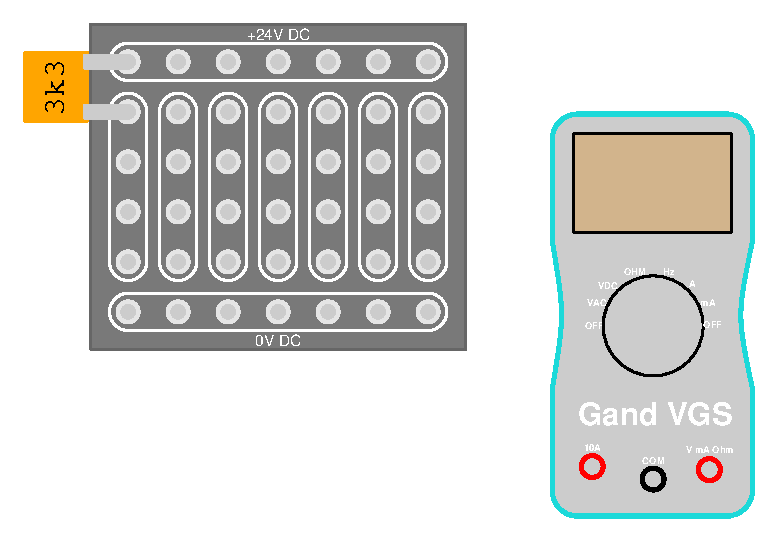
\includegraphics[width=17cm]{./aIndElec01.eps}$$
\vskip 1cm
\vskip 1cm
\end{document}
